\documentclass[a4paper]{article}
\usepackage{unifrrr}
\usepackage{graphicx}
\usepackage[latin1]{inputenc}
\usepackage{float}
\usepackage[colorlinks=false, pdfborder={0 0 0}]{hyperref}
\usepackage{verbatim}
\usepackage{hyperref}
\usepackage{listings}

\setcounter{secnumdepth}{4}
\setcounter{tocdepth}{4}

%--------------------------------------------------------------------


%The body of the LaTeX file
\begin{document}  



%Including of the title page. See titlepage.tex file
%Autor: Daniel Fasel daniel.fasel@unifr.ch
%Date: 10.01.2008
%Comment: An example of a title page file

%Starting the title page. A \begin command always ends with a \end command
\begin{titlepage} 
	%Center all the following stuff
	\begin{center}
		
		%Include the unifr.jpg file from ./images. \\ is a line break
		
\includegraphics[scale=2]{images/unifr.jpg}\\
		
		%Do a vertical space of 0.5 cm
		\vspace{0.5cm}
		
		
	
		\vspace{2cm}
		
		\begin{Large}
		Seminar Thesis: Applying Fuzzy Logic to Data Warehouses\\
		\end{Large}
		
		\vspace{2cm}
		
		%Start a huge font
		\begin{huge}
			%Sans serif
			{\sf \bf Fuzzy Concepts on Real Time Applications}
		\end{huge}
		
				
		\vspace{2cm}
		
		 %N\"uesch in capitals
		 Steve ASCHWANDEN \\
		 Stefan \textsc{N\"UESCH}\\
		
		\vspace{1.5cm}
		
		{\bf Examiner}\\
		Dr. Daniel Fasel\\
		\vspace{2.5cm}
		
		
		Wabern, \today\\
		
				
	\end{center}
\end{titlepage}


\pagenumbering{arabic}
\pagestyle{plain}
\newpage

\section{Introduction}

The number of new tweets per second on the social media platform Twitter\footnote{https://www.twitter.com} is huge (over hundred thousand per second). To handle such a big amount of data, a scalable, fault-tolerant real-time framework has to be used. Storm was benchmarked at processing one million 100 byte messages per second per node\footnote{http://storm-project.net}. It allows to classify every new tweet, for example with a fuzzy logic approach. The so called ''Spout'' is responsible for fetching the tweets and the ''Bolts'' can do some transformation on the received data or persist them in some sort of storage. Cassandra\footnote{http://cassandra.apache.org} is an ideal solution for the given scenario, because it is a distributed, elastically scalable, highly available, fault-tolerant and column-oriented database.

\section{Problem Statement}

\subsection{Research Questions}
\vspace{0.5cm}
\begin{itemize}
\item How can fuzzy classifications be applied to twitter feeds using storm?
\item How can the results of such classifications be stored in a cassandra column store?
\end{itemize}



\section{Objectives}

The main objective of this seminar project is to develop a simple prototype, which uses storm to fuzzily classify messages from twitter feeds and store the results in a Cassandra NoSQL database.
The resulting application will use Storm on local system only (not on a cluster). Furthermore, only one fuzzy concept will be implemented in combination with a simple semantic analysis of the twitter feeds. However, the prototype shall be easily extensible with more complex analytics and further fuzzy concepts.


\section{Methodology}
This thesis will be conducted by prototyping. 
\subsection{Prototype}
The prototype resulting from this project will be a Java application based on the Storm library and using Cassandra for persistence. For analysing the twitter feeds, SentiWordNet will be used. 

\section{Existing Research}
\subsection{Twitter \& Storm}
Storm is an open source distributed real-time computation system and programming language independent. A storm topology consists of two main components:
\begin{itemize}
	\item Spouts are responsible to fetch the data from a source (e.g. text file, twitter streaming API)
	\item Bolts are responsible for the transformations of the fetched data
\end{itemize}
The spout acts as the source of the data flow and the last bolt is the sink which store the output to a database. The output of one component goes always to the input of the next, therefore no data will flow through an already visited node. To illustrate the components of the storm architecture we will take a look at the following example:\\\\
All the spoken words during the TV news show will be stored in a text file. If a new sentence was written into the file the spout hands them to the responsible bolt which separate the sentence into words. This stream of words is passed to another bolt that compares each word to a list of politician's names. If there is a match, the second bolt increases the counter for that name in a storage. To check the number of occurrence, query the database which is updated in real-time.\\
Figure 1.1 Storm book\\
In a storm cluster there are 2 node types, a master node and worker nodes. On the master node runs a daemon called 'Nimbus', which is responsible for code distribution, assigning tasks to the worker nodes and failure monitoring. A portion of the topology is running on the worker nodes (responsible daemon is called 'Supervisor'). A topology runs across multiple worker nodes on different machines. All the daemons are stateless and can fail or restart without disturbing the system.\\
Storm topologies can run in two different modes. The local mode is a single Java Virtual Machine on a local machine. This mode is used for developing, testing and debugging. The other possibility is to run the software on different remote machines. But there are no debugging information in the production mode.\\
The difference between a traditional BigData approach like Hadoop and storm is the paradigm that it addresses. Hadoop fundamentally a batch processing system. The results are available after the whole data was distributed over the whole system. The construction of topologies that transform unterminated streams of data is supported by storm. A storm topology will never stop running (until termination by user), Hadoop jobs will stop after all available data (at starting time) proceeded by the system.

\subsection{Storm with Cassandra}
\subsection{SentiWordNet}

\section{Implementation}
\subsection{Architecture}
\subsection{SentiWordNet Analysis}
SentiNetWord is an English dictionary for opinion mining (OM, also known as sentiment classification). The goal was to decide for every word of the WordNet if it has a positive, negative or neutral meaning. WordNet is a large lexical database of nouns, verbs, adjectives and adverbs provided by the Princeton University. The developers calculated for every word three values between 0.0 and 1.0 and they had to sum up to one. They labelled different entries of the dictionary manually to define a ground truth for the training set. Then a set of classifiers was trained with the provided data. After these steps the classifiers were able to calculate the corresponding values of the remaining words which weren't in the training data samples. Since the first version of SentiWordNet in 2006 a lot of improvements are done, the actual version is 3.0.0. It's freely available for research approaches.\\
The dictionary consists of 117'659 entries (69.8\% nouns, 15.4\% adjectives, 11.7\% verbs and 3.1\% adverbs). If we take a closer look at the calculated values (in SentiNetWord 1.0.0) we can see that most of the words are objective (about eighty percent are greater than 0.75). Only a few words are positive (0.48\% \textgreater \ 0.75; about 560 words) or negative (1.28\% \textgreater \ 0.75; about 1500 words).\\
The resulting dictionary can be downloaded on the research website of SentiWordNet and has the following columns (tab separated):
\begin{enumerate}
	\item Part of speech (noun, verb, adjective, adverb)
  \item ID
	\item Positive score
	\item Negative score
	\item The words (plural because of synonyms)
	\item Glossary (the word in a given context)
\end{enumerate}
The neutral (objective) score of the word can be calculated by 1 - (Positive score + Negative score).

\subsection{Fuzzy Concept Implementation}
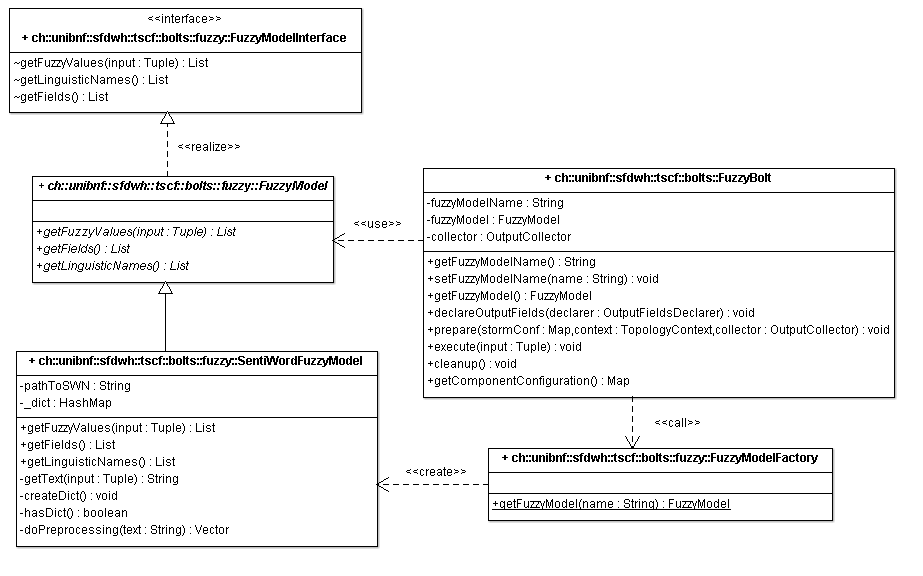
\includegraphics[scale=0.5]{images/FuzzyModelFactory_Diagram.png}\\
To delegate the creation of the model with the implemented fuzzy approach to the \textit{FuzzyBolt} class, a Parameterized Factory Method pattern is used. It's possible to create a new fuzzy model approach by extending the \textit{FuzzyModel} class and modify the \textit{FuzzyModelFactory} to make the object creation of the corresponding model accessible. The selection of the new approach can be done by the following statements:
\lstset{language=Java}
\begin{lstlisting}
FuzzyBolt fuzzyBolt = new FuzzyBolt();
fuzzyBolt.setFuzzyModelName(``our approach'');
\end{lstlisting}
The second line will call the static \textit{getFuzzyModel} method of the factory.
The \textit{SentiWordFuzzyModel} class has a \textit{createDict} method which creates a hash map out of the text file consists of the word as key and the corresponding vector with the opinions (positive, negative and neutral) as value.
The \textit{FuzzyBolt} class is the first bolt in the whole Storm process and receives the output of the twitter spout. The execute-method calculates the three sentiment values of the tweet and give them to the Cassandra bolt.

\section{Conclusion}



\section{References}
\bibliography{diva_group}
\bibliographystyle{plain}

\addcontentsline{Tc}{section}{Bibliography}

\begin{thebibliography}{20}

	\bibitem{senti}
	Andrea Esuli, Fabrizio Sebastiani
	\newblock{\em SentiWordNet: A Publicly Available Lexical Resource for Opinion Mining}
	\newblock available: \url{http://sentiwordnet.isti.cnr.it/}, accessed 18th November 2013.
	
	\bibitem{senti3}
	Stefano Baccianella, Andrea Esuli, Fabrizio Sebastiani
	\newblock{\em SentiWordNet 3.0: An Enhanced Lexical Resource for Sentiment Analysis and Opinion Mining}
	\newblock available: \url{http://sentiwordnet.isti.cnr.it/}, accessed 18th November 2013.
	
	\bibitem{twitter}
	Alec Go, Lei Huang, Richa Bhayani
	\newblock{\em Twitter Sentiment Analysis}
	\newblock available: \url{http://www-nlp.stanford.edu/courses/cs224n/2009/fp/3.pdf}, accessed 18th November 2013.
	
	\bibitem{twitterStorm}
	M. Tim Jones
	\newblock{\em Process real-time big data with Twitter Storm}
	\newblock available: \url{http://www.ibm.com/developerworks/library/os-twitterstorm/os-twitterstorm-pdf.pdf}, accessed 18th November 2013.
	
	\bibitem{stormCassandra}
	Shalom N. 
	\newblock{\em Nati Shalom's Blog: Real-Time Big Data with Storm, Cassandra, and XAP; April 4th, 2013}
	\newblock available: \url{http://natishalom.typepad.com/nati_shaloms_blog/2013/04/real-time-big-data-with-storm-cassandra-and-xap-1.html}, accessed 18th November 2013.

	\bibitem{stormBook}
	Jonathan Leibiusky, Gabriel Eisbruch and Dario Simonassi 
	\newblock{\em Getting Started with Storm;}
	\newblock 30th August 2012; O'Reilly, 978-1-449-32401-8

	\bibitem{cassandraBook}
	Eben Hewitt 
	\newblock{\em Cassandra - The Definitive Guide;}
	\newblock November 2010; O'Reilly, 978-1-449-39041-9
	
	\newblock{}
	\newblock{}
	
		
\end{thebibliography}




\end{document}
